\newcommand{\installerTagResultsAucTable}{
    \begin{table}[H]
        \centering
        \begin{tabular}{|p{2,8cm}||p{2,8cm} p{2,8cm} p{2,8cm}|}
            \hline
            Installer Tag & ALOHA & Joint Embedding & Proposed Model \\
            \hline
            AUC-ROC & 0.552$\pm$0.010 & \textBF{0.576$\pm$0.012} & 0.564$\pm$0.005 \\
            \hline
        \end{tabular}
        \caption{AUC-ROC (Area Under Curve) of the different models for the \textbf{Installer Tag} prediction task. Results were aggregated over \textBF{3} training runs with different weight initializations and minibatch orderings. Best results are shown in \textbf{bold}.} \label{tab:installerTag_auc}
    \end{table}
}

\newcommand{\installerTagResultsAtFprTable}{
    \begin{center}
        \begin{longtable}[c]{|p{3,2cm}||p{1,8cm} p{1,8cm} p{1,8cm} p{1,8cm} p{1,8cm}|}
            \hline
            Installer Tag & \multicolumn{5}{c|}{{FPR}} \\
            & $10^{-5}$ & $10^{-4}$ & $10^{-3}$ & $10^{-2}$ & $10^{-1}$ \\
            \hline
            \endfirsthead

            \caption*{\raggedright ...continued from previous page} \\
            \hline
            Installer Tag & \multicolumn{5}{c|}{\textbf{FPR}} \\
            & $10^{-5}$ & $10^{-4}$ & $10^{-3}$ & $10^{-2}$ & $10^{-1}$ \\
            \hline
            \endhead

            \caption*{\raggedleft ...continued on next page} \\
            \endfoot

            \caption{Mean and standard deviation results (TPR, Accuracy, Recall, Precision and F1-Score) of the different models for the \textbf{Installer Tag} prediction task at different \textbf{FPR}s (\textit{False Positive Rates}). Results were aggregated over \textBF{3} training runs with different weight initializations and minibatch orderings. Best results are shown in \textbf{bold}. Under \textbf{TPR} results are also presented the percentage reduction in mean detection error and in ROC curve standard deviation introduced by the \textit{Proposed Model} with respect to both \textit{ALOHA} model and \textit{Joint Embedding}.} \label{tab:installerTag_results_at_fpr} \\
            \endlastfoot

            \multicolumn{6}{|c|}{\textbf{TPR}} \\
            \hline
            ALOHA & 0.000$\pm$0.000 & 0.000$\pm$0.000 & 0.000$\pm$0.000 & 0.014$\pm$0.012 & 0.095$\pm$0.018 \\
            Joint Embedding & \textBF{0.005$\pm$0.007} & \textBF{0.005$\pm$0.007} & \textBF{0.010$\pm$0.007} & \textBF{0.029$\pm$0.012} & \textBF{0.152$\pm$0.013} \\
            Proposed Model & 0.000$\pm$0.000 & 0.000$\pm$0.000 & 0.005$\pm$0.007 & 0.014$\pm$0.012 & 0.138$\pm$0.018 \\
            \hline
            Error Reduction wrt \newline ALOHA & 0.0\% & 0.0\% & 0.5\% & 0.0\% & 4.8\% \\
            Error Reduction wrt \newline Joint Embedding & -0.5\% & -0.5\% & -0.5\% & -1.5\% & -1.7\% \\
            \hline
            Std Reduction wrt \newline ALOHA & 0.0\% & 0.0\% & 0.0\% & 0.0\% & 0.0\% \\
            Std Reduction wrt \newline Joint Embedding & 100.0\% & 100.0\% & 0.0\% & 0.0\% & -38.5\% \\
            \hline
            \multicolumn{6}{|c|}{\textbf{Accuracy}} \\
            \hline
            ALOHA & 0.971$\pm$0.000 & 0.971$\pm$0.000 & \textBF{0.971$\pm$0.000} & 0.965$\pm$0.003 & 0.877$\pm$0.001 \\
            Joint Embedding & \textBF{0.972$\pm$0.000} & \textBF{0.972$\pm$0.000} & 0.971$\pm$0.001 & 0.964$\pm$0.001 & \textBF{0.879$\pm$0.001} \\
            Proposed Model & 0.971$\pm$0.000 & 0.971$\pm$0.000 & \textBF{0.971$\pm$0.000} & \textBF{0.966$\pm$0.002} & \textBF{0.879$\pm$0.001} \\
            \hline
            \multicolumn{6}{|c|}{\textbf{Recall}} \\
            \hline
            ALOHA & 0.000$\pm$0.000 & 0.000$\pm$0.000 & 0.000$\pm$0.000 & 0.014$\pm$0.012 & 0.095$\pm$0.018 \\
            Joint Embedding & \textBF{0.005$\pm$0.007} & \textBF{0.005$\pm$0.007} & \textBF{0.010$\pm$0.007} & \textBF{0.029$\pm$0.012} & \textBF{0.152$\pm$0.013} \\
            Proposed Model & 0.000$\pm$0.000 & 0.000$\pm$0.000 & 0.005$\pm$0.007 & 0.014$\pm$0.012 & 0.138$\pm$0.018 \\
            \hline
            \multicolumn{6}{|c|}{\textbf{Precision}} \\
            \hline
            ALOHA & \textBF{1.000$\pm$0.000} & \textBF{1.000$\pm$0.000} & 0.000$\pm$0.000 & 0.041$\pm$0.033 & 0.027$\pm$0.005 \\
            Joint Embedding & \textBF{1.000$\pm$0.000} & \textBF{1.000$\pm$0.000} & \textBF{0.444$\pm$0.416} & \textBF{0.088$\pm$0.032} & \textBF{0.043$\pm$0.004} \\
            Proposed Model & \textBF{1.000$\pm$0.000} & \textBF{1.000$\pm$0.000} & 0.111$\pm$0.157 & 0.049$\pm$0.035 & 0.039$\pm$0.005 \\
            \hline
            \multicolumn{6}{|c|}{\textbf{F1 Score}} \\
            \hline
            ALOHA & 0.000$\pm$0.000 & 0.000$\pm$0.000 & 0.000$\pm$0.000 & 0.021$\pm$0.017 & 0.042$\pm$0.008 \\
            Joint Embedding & \textBF{0.009$\pm$0.013} & \textBF{0.009$\pm$0.013} & \textBF{0.019$\pm$0.013} & \textBF{0.043$\pm$0.017} & \textBF{0.067$\pm$0.006} \\
            Proposed Model & 0.000$\pm$0.000 & 0.000$\pm$0.000 & 0.009$\pm$0.013 & 0.022$\pm$0.017 & 0.061$\pm$0.008 \\
            \hline
        \end{longtable}
    \end{center}
}

\newcommand{\installerTagResultsSummaryTable}{
    \begin{table}[H]
        \centering
        \begin{tabular}{|p{3,2cm}||p{1,8cm} p{1,8cm} p{1,8cm} p{1,8cm} p{1,8cm}|}
            \hline
            \multicolumn{6}{|c|}{Installer Tag (at FPR $=1\%$)} \\
            \hline
            Model & TPR & Accuracy & Precision & Recall & F1 score \\
            \hline
            ALOHA & 0.014$\pm$0.012 & 0.965$\pm$0.003 & 0.041$\pm$0.033 & 0.014$\pm$0.012 & 0.021$\pm$0.017 \\
            Joint Embedding & \textBF{0.029$\pm$0.012} & 0.964$\pm$0.001 & \textBF{0.088$\pm$0.032} & \textBF{0.029$\pm$0.012} & \textBF{0.043$\pm$0.017} \\
            Proposed Model & 0.014$\pm$0.012 & \textBF{0.966$\pm$0.002} & 0.049$\pm$0.035 & 0.014$\pm$0.012 & 0.022$\pm$0.017 \\
            \hline
        \end{tabular}
        \caption{Summary of the mean and standard deviation results of the different models for the \textbf{Installer Tag} prediction task at \textbf{FPR} $=1\%$. Results were aggregated over \textBF{3} training runs with different weight initializations and minibatch orderings. Best results are shown in \textbf{bold}.} \label{tab:installerTag_result_summary}
    \end{table}
}

\newcommand{\installerTagRocAloha}{
    \begin{figure}[H]
        \centering
        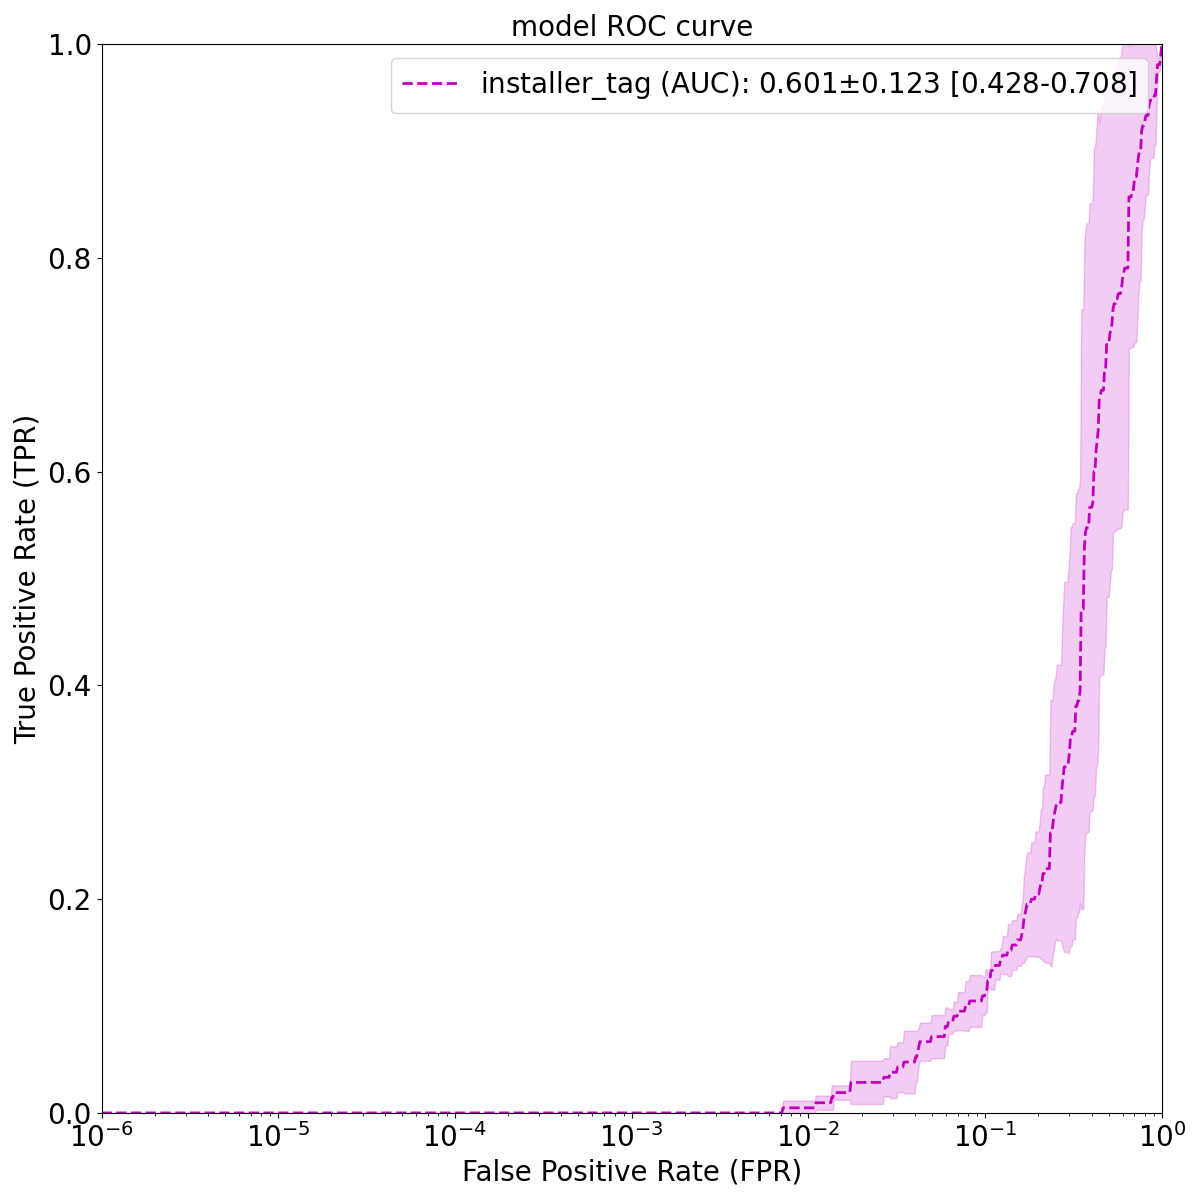
\includegraphics[width=0.8\textwidth]{./results/installer_tag_roc_aloha.png}
        \vspace*{-1cm}
        \caption{ROC curve and AUC statistics of \textBF{ALOHA} model for the \textbf{Installer Tag}. The line represents the \textit{mean} TPR at a given FPR, while the shaded region represents the \textit{standard deviation}. Statistics were computed over \textBF{3} training runs, each with random parameter initialization.}
        \label{fig:installerTagRocAloha}
    \end{figure}
}

\newcommand{\installerTagRocJointEmbedding}{
    \begin{figure}[H]
        \centering
        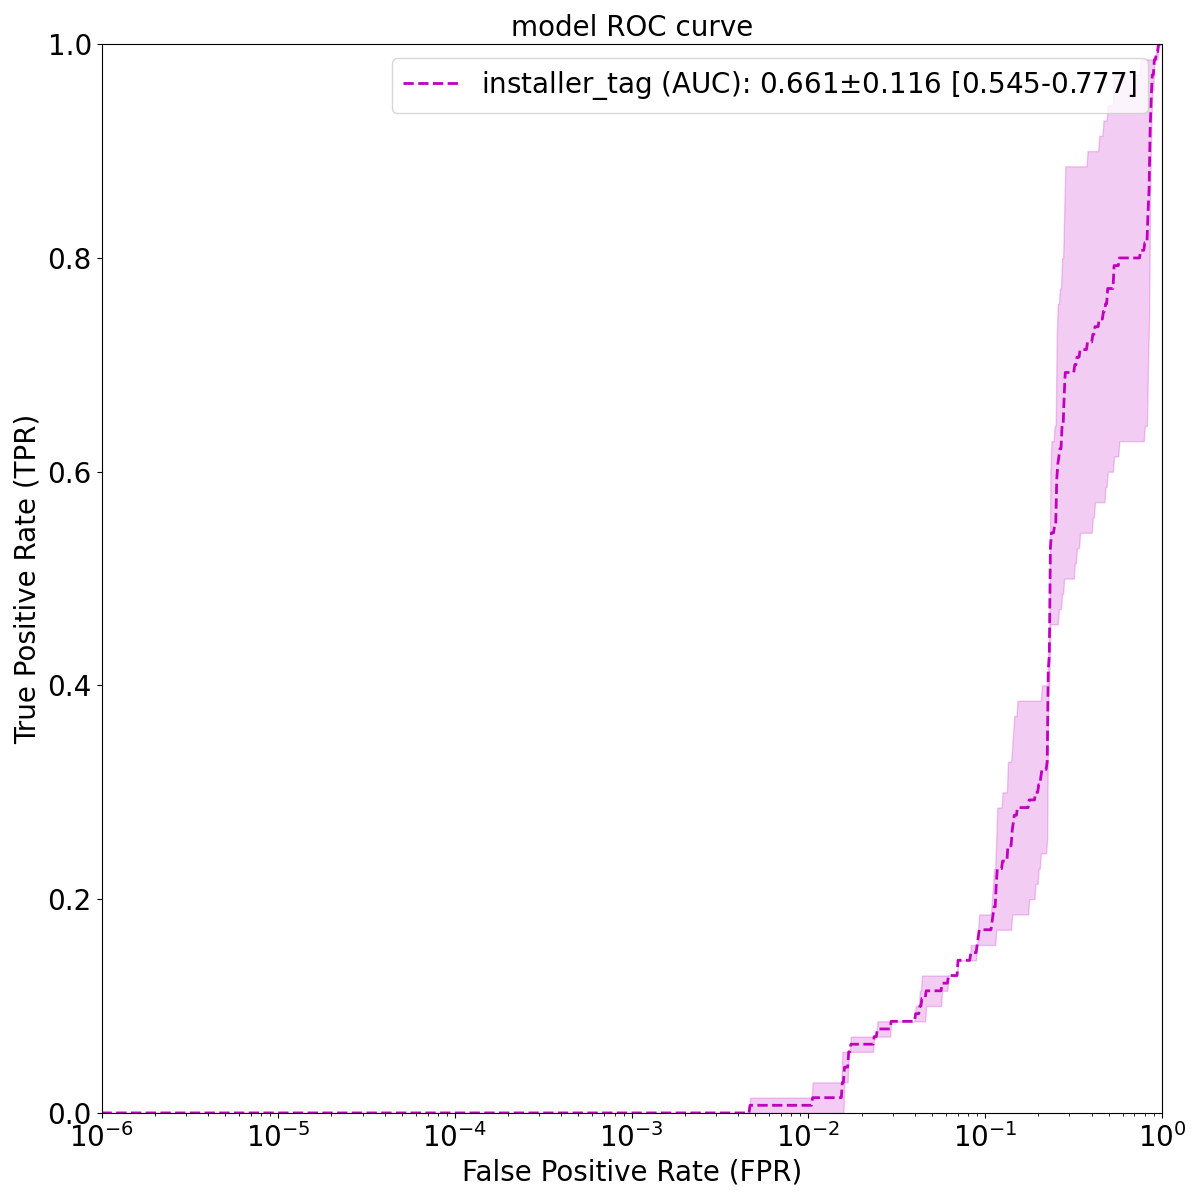
\includegraphics[width=0.8\textwidth]{./results/installer_tag_roc_jointEmbedding.png}
        \vspace*{-1cm}
        \caption{ROC curve and AUC statistics of \textBF{Joint Embedding} model for the \textbf{Installer Tag}. The line represents the \textit{mean} TPR at a given FPR, while the shaded region represents the \textit{standard deviation}. Statistics were computed over \textBF{3} training runs, each with random parameter initialization.}
        \label{fig:installerTagRocJointEmbedding}
    \end{figure}
}

\newcommand{\installerTagRocProposedMethod}{
    \begin{figure}[H]
        \centering
        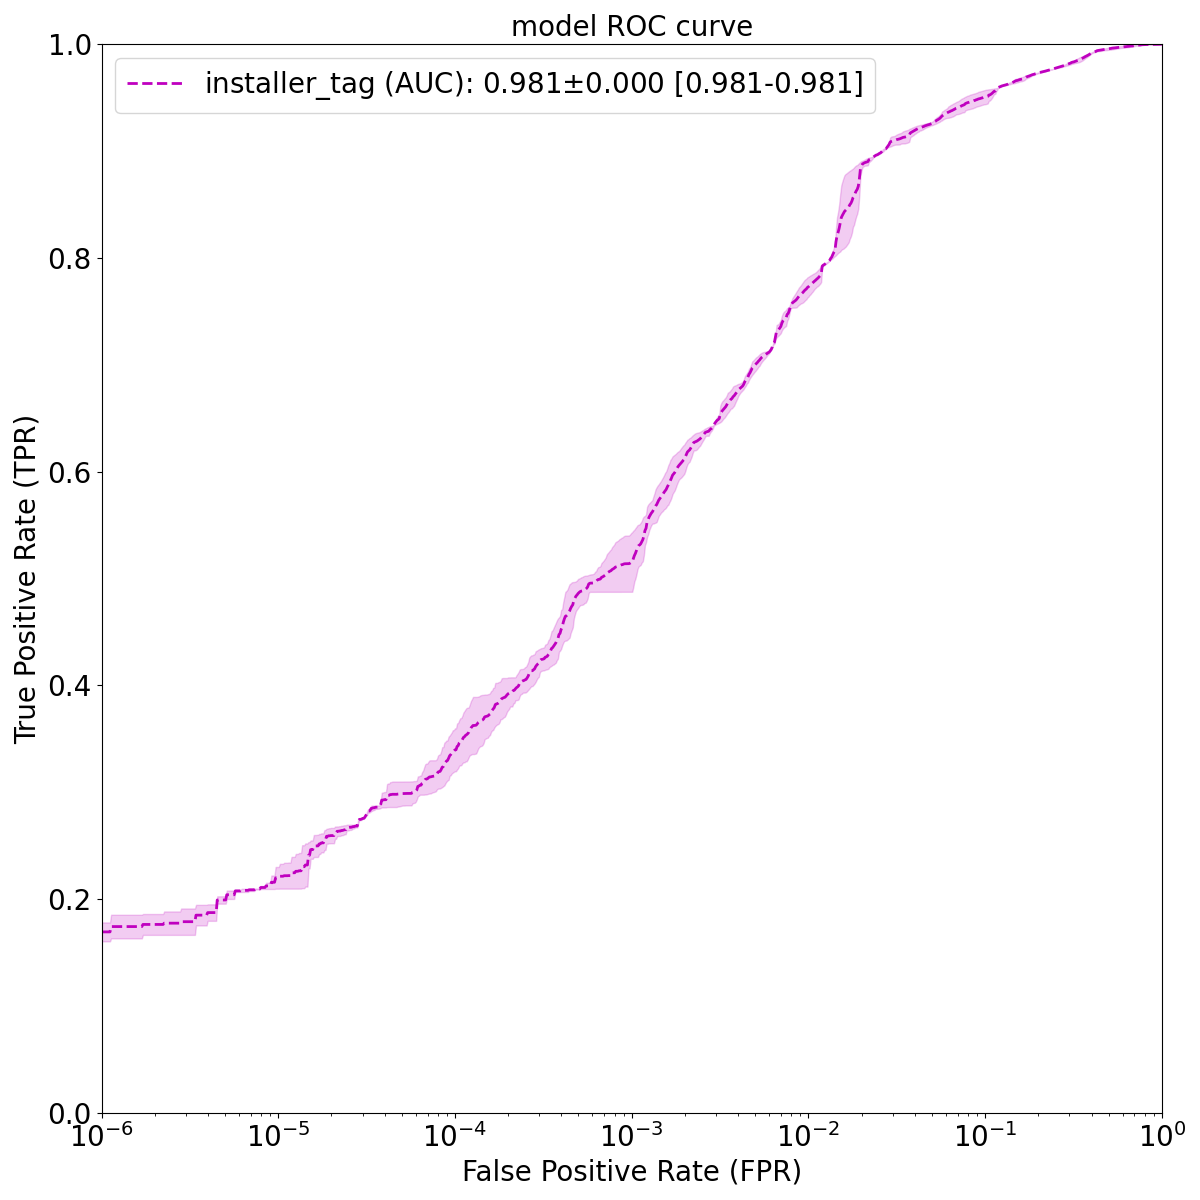
\includegraphics[width=0.8\textwidth]{./results/installer_tag_roc_proposedModel.png}
        \vspace*{-1cm}
        \caption{ROC curve and AUC statistics of \textBF{Proposed Model} for the \textbf{Installer Tag}. The line represents the \textit{mean} TPR at a given FPR, while the shaded region represents the \textit{standard deviation}. Statistics were computed over \textBF{3} training runs, each with random parameter initialization.}
        \label{fig:installerTagRocProposedModel}
    \end{figure}
}
